%%%%%%%%%%%%%%%%%%%%%%%%%%%%%%%%%%%%%%%
\section{Capture-recapture experiments}
\begin{slide}\slidetitle{Capture-recapture experiments}
\tableofcontents[sectionstyle=show/hide,subsectionstyle=show/shaded/hide]

\end{slide}
%%%%%%%%%%%%%%%%%%%%%%%%%%%%%%%%%%%%%%%
\subsection{Inference in finite populations}
\begin{slide}\slidetitle{Inference in finite populations}

\normalsize 
Problem of estimating an unknown population size, $N$, based on
partial observation of this population: domain of {\em survey
sampling} 

\begin{block}{Warning}
We do not cover the official Statistics/stratified type of survey based on
a preliminary knowledge of the structure of the population
\end{block}

\end{slide}\begin{slide} 
\slidetitle{Numerous applications}

\begin{itemize}
\item \MidnightBlue{{\em Biology \&\ Ecology}} 
	for estimating the size of herds, of fish or whale populations, etc.
\pause
\item \MidnightBlue{{\em Sociology \&\ Demography}} 
	for estimating the size of populations at risk, including 
	homeless people, prostitutes, illegal migrants, drug addicts, etc.
\pause
\item \MidnightBlue{{\em official Statistics}} in the U.S.~and French census undercount procedures
\item \MidnightBlue{{\em Economics \&\ Finance}} in credit scoring, defaulting companies, etc.,
\pause
\item \MidnightBlue{{\em Fraud detection}}  phone, credit card, etc.
\item \MidnightBlue{{\em Document authentication}} historical documents, forgery, etc.,
\item \MidnightBlue{{\em Software debugging}}
\end{itemize}

\end{slide}\begin{slide} 
\slidetitle{Setup}

Size $N$ of the whole population is unknown
but samples (with fixed or random sizes) can 
be extracted from the population. 

%%%%%%%%%%%%%%%%%%%%%%%%%%%%%%%%%%%%%%%
\end{slide}\subsection{Binomial capture model}\begin{slide}
\slidetitle{The binomial capture model}

Simplest model of all: joint capture of $n^+$ individuals from a population of size $N$.

\vs\pause Population size $N\in\mathbb{N}^*$ is the parameter of interest, but there exists a
nuisance  parameter, the probability $p\in[0,1]$ of capture [under assumption of independent captures]

\vs\pause
Sampling model
$$
n^+ \sim \mathscr{B}(N,p)
$$
and corresponding likelihood 
$$
\ell(N,p|n^+)={N \choose n^+}\,p^{n^+}(1-p)^{N-n^+}\mathbb{I}_{N\ge n^+}\,.
$$

\end{slide}\begin{slide}
\slidetitle{Bayesian inference (1)}
Under vague prior
$$
\pi(N,p)\propto N^{-1}\mathbb{I}_{\mathbb{N}^*}(N)\mathbb{I}_{[0,1]}(p)\,,
$$
posterior distribution of $N$ is 
\small\begin{eqnarray*}
\pi(N|n^+) & \propto & \frac{N!}{(N-n^+)!}\,N^{-1}\mathbb{I}_{N\ge n^+}\mathbb{I}_{\mathbb{N}^*}(N)\int_0^1 p^{n^+}(1-p)^{N-n^+}dp \\
           & \propto & \frac{(N-1)!}{(N-n^+)!}\,\frac{(N-n^+)!}{(N+1)!}\,\mathbb{I}_{N\geq n^+\vee 1} \\
           & =       & \frac{1}{N(N+1)}\mathbb{I}_{N\geq n^+\vee 1}\,.
\end{eqnarray*}
\normalsize where $n^+\vee 1=\max(n^+,1)$

\end{slide}\begin{slide}
\slidetitle{Bayesian inference (2)}
If we use the uniform prior
$$
\pi(N,p)\propto \mathbb{I}_{\{1,\ldots,S\}}(N)\mathbb{I}_{[0,1]}(p)\,,
$$
the posterior distribution of $N$ is
$$
\pi(N|n^+)\propto \frac{1}{N+1}\mathbb{I}_{\{n^+\vee 1,\ldots,S\}}(N)\,.
$$

\end{slide}
\begin{slide}
\slidetitle{Capture-recapture data}

\begin{block}{European dippers}
\begin{columns}\column{.55\textwidth}
Birds closely dependent on streams, feeding on underwater invertebrates

Capture-recapture data on dippers over  years 1981--1987
in $3$ zone of $200$ $\text{km}^2$ in eastern France with markings and recaptures
of breeding adults each year, during the breeding period from early March to early June.
\column{.35\textwidth}

\includegraphics[width=3cm,height=3truecm]{figures/Dipper.eps}
\end{columns}
\end{block}

\end{slide}
\begin{frame}[fragile]
\frametitle{{\sf eurodip}}

Each row of $7$ digits corresponds to a capture-recapture story: 
$0$ stands for absence of capture and, else,
$1,2$ or $3$ represents the zone of capture.

\vs\pause
E.g.
\begin{verbatim}
1 0 0 0 0 0 0
1 3 0 0 0 0 0
0 2 2 2 1 2 2
\end{verbatim}
means: first dipper only captured the first year [in zone 1], second dipper
captured in years 1981--1982 and moved from zone 1 to zone 3 between those years, third dipper
captured in years 1982--1987 in zone 2

\end{frame}
%%%%%%%%%%%%%%%%%%%%%%%%%%%%%%%%%%%%%%%
\subsection{Two-stage capture-recapture}\begin{slide}
\slidetitle{The two-stage capture-recapture experiment}

Extension to the above with two capture periods plus a marking stage:
\begin{enumerate}
\item  $n_1$ individuals from a population of size $N$ captured {\em [sampled without replacement]}
\item  captured individuals marked and released
\item  $n_2$ individuals captured during second identical sampling experiment
\item  $m_2$ individuals out of the $n_2$'s bear the identification mark {\em [captured twice]}
\end{enumerate}

\end{slide}\begin{slide}
\slidetitle{The two-stage capture-recapture model}

For {\em closed populations} [fixed population size $N$ throughout
experiment, constant capture probability $p$ for all individuals, and independence between
individuals/captures], binomial models:
\pause
$$
n_1     \sim\mathscr{B}(N,p)\,,\quad
m_2|n_1 \sim\mathscr{B}(n_1,p)\quad\hbox{and}
$$
$$
n_2-m_2|n_1,m_2 \sim\mathscr{B}(N-n_1,p)\,.
$$

\end{slide}\begin{slide}
\slidetitle{The two-stage capture-recapture likelihood}

Corresponding likelihood $\ell(N,p|n_1,n_2,m_2)$
\small\begin{align*}
{N-n_1 \choose n_2-m_2} &p^{n_2-m_2}(1-p)^{N-n_1-n_2+m_2} \mathbb{I}_{\{0,\ldots,N-n_1\}}(n_2-m_2)\\
                      &\times  {n_1 \choose m_2}p^{m_2}(1-p)^{n_1-m_2}{N \choose n_1}p^{n_1}(1-p)^{N-n_1} \mathbb{I}_{\{0,\ldots,N\}}(n_1) \\
                      &\propto \frac{N!}{(N-n_1-n_2+m_2)!} p^{n_1+n_2}(1-p)^{2N-n_1-n_2}\mathbb{I}_{N\geq n^+} \\
                      &\propto {N \choose n^+}p^{n^c}(1-p)^{2N-n^c}\mathbb{I}_{N\geq n^+}
\end{align*}
\normalsize where $n^c=n_1+n_2$ and $n^+=n_1+(n_2-m_2)$ are
total number of captures/captured individuals over both periods 

\end{slide}\begin{slide}
\slidetitle{Bayesian inference (1)}

Under prior $\pi(N,p)=\pi(N)\pi(p)$ where $\pi(p)$ is  $\mathscr{U}([0,1])$, 
conditional posterior distribution on $p$ is
$$
\pi(p|N,n_1,n_2,m_2)=\pi(p|N,n^c)\propto p^{n^c}(1-p)^{2N-n^c}\,,
$$
that is,
$$
p|N,n^c\sim\mathscr{B}e(n^c+1,2N-n^c+1).
$$

\vs\pause
Marginal posterior distribution of $N$ more complicated. 
If $\pi(N)=\mathbb{I}_{\mathbb{N}^*}(N)$, 
$$
\pi(N|n_1,n_2,m_2)\propto {N \choose n^+}B(n^c+1,2N-n^c+1)\mathbb{I}_{N\geq n^+\vee 1}
$$
{\em [Beta-Pascal distribution]}

\end{slide}\begin{slide}
\slidetitle{Bayesian inference (2)}

Same problem if $\pi(N)=N^{-1}\mathbb{I}_{\mathbb{N}^*}(N)$. 

\begin{block}{Computations}
Since $N\in\mathbb{N}$, always possible to approximate the missing
normalizing factor in $\pi(N|n_1,n_2,m_2)$ by summing in $N$. 

Approximation errors become a problem when $N$ and $n^+$ are large.
\end{block}

\vs\pause
Under proper uniform prior,
$$
\pi(N)\propto \mathbb{I}_{\{1,\ldots,S\}}(N)\,,
$$
posterior distribution of $N$ proportional to
$$
\pi(N|n^+)\propto {N \choose n^+}\frac{\Gamma(2N-n^c+1)}{\Gamma(2N+2)}\,\mathbb{I}_{\{n^+\vee 1,\ldots,S\}}(N)\,.
$$
and can be computed with no approximation error.

\end{slide}\begin{slide}
\slidetitle{The Darroch model}

Simpler version of the above: conditional on both samples sizes $n_1$ and $n_2$,
$$
m_2|n_1,n_2 \sim \mathscr{H}(N,n_2,n_1/N)\,.
$$

Under uniform prior on $N\sim\mathscr{U}(\{1,\ldots,S\})$,
posterior distribution of $N$
$$
\pi(N|m_2) \propto {n_1 \choose m_2} {N-n_1\choose n_2-m_2} \bigg/ {N\choose n_2}\mathbb{I}_{\{n^+\vee 1,\ldots,S\}}(N)
$$
and posterior expectations computed numerically by simple summations.
\end{slide}\begin{slide}
\slidetitle{{\sf eurodip}}

For the two first years and $S=400$,
posterior distribution of $N$
for the Darroch model given by
$$
\pi(N|m_2) \propto (n-n_1)!(N-n_2)!\big/\{(n-n_1-n_2+m_2)!N!\}\,\mathbb{I}_{\{71,\ldots,400\}}(N)\,,
$$
with inverse normalization factor 
$$
\sum_{k=71}^{400} (k-n_1)!(k-n_2)!\big/\{(k-n_1-n_2+m_2)!k!\}\,.
$$

\pause Influence of prior hyperparameter $S$ (for $m_2=11$):

\small
\begin{center}\begin{tabular}{ c|c c c c c c c c c }
%\hline
$S$ & $100$ & $150$ & $200$ & $250$ & $300$ & $350$ & $400$ & $450$ & $500$ \cr
\hline
$\mathbb{E}[N|m_2]$ & $95$ & $125$ & $141$ & $148$  & $151$ & $151$ & $152$ & $152$ & $152$ \cr
%\hline
\end{tabular}\end{center}
\normalsize

\end{slide}\begin{slide}
\slidetitle{Gibbs sampler for $2$-stage capture-recapture}

If $n^+>0$, both conditional posterior distributions are standard, since
\begin{eqnarray*}
p|n^c,N      & \sim & \mathscr{B}e(n^c+1,2N-n^c+1) \\
N-n^+|n^+,p  & \sim & \mathscr{N}eg(n^+,1-(1-p)^2)\,.
\end{eqnarray*}

Therefore, joint distribution of $(N,p)$ can be approximated by a Gibbs sampler

%%%%%%%%%%%%%%%%%%%%%%%%%%%%%%%%%%%%%%%
\end{slide}\begin{slide}
\slidetitle{$T$-stage capture-recapture model}

Further extension to the two-stage capture-recapture model: series of $T$ consecutive captures.

$n_t$ individuals captured at period $1\le t\le T$, and $m_t$ recaptured individuals (with the convention that $m_1=0$) 
$$
n_1\sim\mathscr{B}(N,p)
$$
and, conditional on earlier captures/recaptures $(2\le j\le T)$,
\begin{align*}
m_j&\sim\mathscr{B}\left(\sum_{t=1}^{j-1}(n_t-m_t),p\right)\quad\hbox{and}\\
n_j-m_j&\sim\mathscr{B}\left(N-\sum_{t=1}^{j-1}(n_t-m_t),p\right)\,.
\end{align*}

\end{slide}\begin{slide}
\slidetitle{$T$-stage capture-recapture likelihood}

Likelihood $\ell(N,p|n_1,n_2,m_2\ldots,n_T,m_T)$ given by
\small\begin{align*}
{N \choose n_1} & p^{n_1}(1-p)^{N-n_1} \prod_{j=2}^T\left[{N-{\sum_{t=1}^{j-1}}(n_t-m_t) 
\choose n_j-m_j}\right. p^{n_j-m_j}\\
& \times (1-p)^{N-{\sum_{t=1}^{j}}(n_t-m_t)} \left.{{\sum_{t=1}^{j-1}}(n_t-m_t) \choose m_j}\right. \\
& \times \left.p^{m_j}(1-p)^{{\sum_{t=1}^{j-1}}(n_t-m_t)-m_j}\right]\,.
\end{align*}
\normalsize

\end{slide}\begin{slide}
\slidetitle{Sufficient statistics}

Simplifies into
$$
\ell(N,p|n_1,n_2,m_2\ldots,n_T,m_T) \propto \frac{N!}{(N-n^+)!}p^{n^c}(1-p)^{TN-n^c}\mathbb{I}_{N\geq n^+}
$$
with the sufficient statistics 
$$
n^+=\sum_{t=1}^{T}(n_t-m_t)
\quad\hbox{and}\quad
n^c=\sum_{t=1}^Tn_t\,,
$$
total number of captured individuals/captures over the $T$ periods

\end{slide}\begin{slide}
\slidetitle{Bayesian inference (1)}

Under noninformative prior $\pi(N,p) = 1/N$, joint posterior 
\small\begin{eqnarray*}
\pi(N,p|n^+,n^c) & \propto & \frac{(N-1)!}{(N-n^+)!}\, p^{n^c} (1-p)^{TN-n^c}\mathbb{I}_{N\geq n^+\vee 1}\,.
\end{eqnarray*}\normalsize
leads to conditional posterior
\small$$
p|N,n^+,n^c \sim \mathscr{B}e(n^c+1,TN-n^c+1)
$$\normalsize
and marginal posterior 
\small$$
\pi(N|n^+,n^c) \propto {(N-1)! \over (N-n^+)!}\, { (TN-n^c)! \over (TN+1)!}\, \mathbb{I}_{N\ge n^+\vee 1}
$$\normalsize
which is computable {\em [under previous provisions]}.

\vs\pause
Alternative Gibbs sampler also available.
\end{slide}\begin{slide}
\slidetitle{Bayesian inference (2)}

Under prior $N\sim\mathscr{U}(\{1,\ldots,S\})$ and $p\sim\mathscr{U}([0,1])$,
$$
\pi(N|n^+)\propto {N \choose n^+}\,\frac{(TN-n^c)!}{(TN+1)!}\,\mathbb{I}_{\{n^+\vee 1,\ldots,S\}}(N).
$$

\pause\begin{block}{{\sf eurodip}}
For the whole set of observations, $T=7$, $n^+=294$ and  $n^c=519$.

For $S=400$, the posterior expectation of $N$ is equal to $372.89$.

For $S=2500$, it is $373.99$.
\end{block}

\end{slide}\begin{slide} 
\slidetitle{Computational difficulties}

E.g., heterogeneous capture--recapture 
model where individuals are captured at time $1\le t\le T$ with 
probability $p_t$ with both $N$ and the $p_t$'s are unknown. 

\vs\pause
Corresponding likelihood
\begin{align*}
\ell(N,p_1, \ldots,p_T&|n_1,n_2,m_2\ldots,n_T,m_T)\\
&\propto {N!\over (N - n^+)!} \; 
\prod_{t=1}^{T} \; p_{t}^{n_{t}} (1 - p_{t})^{N-n_{t}}.
\end{align*}

\end{slide}\begin{slide}
\slidetitle{Computational difficulties (cont'd)}

Associated prior $N \sim\mathscr{P}(\lambda)$ and
$$
\alpha_{t} = \log \left({p_{t}\big/ 1 - p_{t}}\right)
\sim {\mathscr{N}}(\mu_{t},\sigma^{2}),
$$
where the $\mu_t$'s and $\sigma$ are known.

\pause
Posterior 
\small\begin{eqnarray*}
\pi(\alpha_1,\ldots,\alpha_T,N|,n_1,\ldots,n_T) \; & \propto & {N!\over (N - n^+)!}\,\frac{\lambda^N}{N!}
\; \prod_{t=1}^T (1 + e^{\alpha_{t}})^{-N} \\
&& \times \prod_{t=1}^T \; \exp \left\{\alpha_t n_t
- {1\over 2\sigma^2 } (\alpha_{t} - \mu_{t})^{2} \right\} \,.
\end{eqnarray*}\normalsize
much less manageable computationally. 

%%%%%%%%%%%%%%%%%%%%%%%%%%%%%%%%%%%%%%%
\end{slide}\subsection{Open population}\begin{slide}
\slidetitle{Open populations}

More realistically, population size does not remain fixed over time: 
probability $q$ for each individual to leave the population at each time [or between
each capture episode] 

\vs\pause
First occurrence of missing variable model.

\vs\pause
Simplified version
where only individuals captured during the first experiment are marked and 
their subsequent recaptures are registered.

\end{slide}\begin{slide}
\slidetitle{Working example}

Three successive capture experiments with
\small\begin{align*}
n_1&\sim\mathscr{B}(N,p),\\
r_1|n_1&\sim\mathscr{B}(n_1,q),\\
c_2|n_1,r_1&\sim\mathscr{B}(n_1-r_1,p),\\ 
r_2|n_1,r_1&\sim\mathscr{B}(n_1-r_1,q)\\
c_3|n_1,r_1,r_2&\sim\mathscr{B}(n_1-r_1-r_2,p)
\end{align*}\normalsize
where only $n_1$, $c_2$ and $c_3$ are observed. 

\vs Variables $r_1$ and $r_2$ not available and therefore part of unknowns like
parameters $N$, $p$ and $q$.

\end{slide}\begin{slide}
\slidetitle{Bayesian inference}
Likelihood 
\small
\begin{align*}
{N\choose n_1}&p^{n_1}(1-p)^{N-n_1}\,{n_1\choose r_1}\,q^{r_1}(1-q)^{n_1-r_1}{n_1-r_1\choose c_2}\,p^{c_2}(1-p)^{n_1-r_1-c_2}\\
&{n_1-r_1\choose r_2} q^{r_2}(1-q)^{n_1-r_1-r_2}{n_1-r_1-r_2\choose c_3} p^{c_3}(1-p)^{n_1-r_1-r_2-c_3}
\end{align*}\normalsize
and prior 
$$
\pi(N,p,q)=N^{-1}\mathbb{I}_{[0,1]}(p)\mathbb{I}_{[0,1]}(q)
$$

\end{slide}\begin{slide}
\slidetitle{Full conditionals for Gibbs sampling}

\begin{align*}
\pi(p|N,q,\mathcal{D}^*) &\propto p^{n_+} (1-p)^{u_+}\\
\pi(q|N,p,\mathcal{D}^*) &\propto q^{c_1+c_2}(1-q)^{2n_1-2r_1-r_2}\\
\pi(N|p,q,\mathcal{D}^*) &\propto {(N-1)! \over (N-n_1)!} (1-p)^N \mathbb{I}_{N\ge n_1}\\
\pi(r_1|p,q,n_1,c_2,c_3,r_2) &\propto \frac{(n_1-r_1)!\,q^{r_1}(1-q)^{-2r_1}(1-p)^{-2r_1}}{
        r_1!(n_1-r_1-r_2-c_3)!(n_1-c_2-r_1)!}\\
\pi(r_2|p,q,n_1,c_2,c_3,r_1) &\propto \frac{q^{r_2}[(1-p)(1-q)]^{-r_2}}{
        r_2!(n_1-r_1-r_2-c_3)!}
\end{align*}
where 
\small
\begin{align*}
\mathcal{D}^*&=(n_1,c_2,c_3,r_1,r_2)\\
u_1&=N-n_1,\,u_2=n_1-r_1-c_2,\,u_3=n_1-r_1-r_2-c_3\\
n_+&=n_1+c_2+c_3,\,u_+=u_1+u_2+u_3
\end{align*}

\end{slide}\begin{slide}
\slidetitle{Full conditionals (2)}
\normalsize
Therefore,
\begin{align*}
p|N,q,\mathcal{D}^* &\sim \mathcal{B}e(n_++1, u_++1) \\
q|N,p,\mathcal{D}^* &\sim \mathcal{B}e(r_1+r_2+1, 2n_1-2r_1-r_2+1) \\
N-n_1|p,q,\mathcal{D}^* &\sim \mathcal{N}eg(n_1,p)\\
%m_1|p,q,n_1,n_2,n_3&\sim \mathcal{B}\left(n_1-m_2-n_3,\frac{q}{1+(1-q)(1-p)^2}\right)
r_2|p,q,n_1,c_2,c_3,r_1 &\sim \mathcal{B}\left(n_1-r_1-c_3,\frac{q}{1+(1-q)(1-p)}\right)
\end{align*}

\vs\pause
$r_1$ has a less conventional distribution,  but, since $n_1$ not
extremely large, possible to compute the probability that $r_1$ is equal 
to one of the values in $\{0,1,\ldots,\min(n_1-r_2-c_3,n_1-c_2)\}$.

\end{slide}\begin{slide}
\slidetitle{{\sf eurodip}}

\begin{columns}
\column{.5\textwidth}
$n_1=22$, $c_2=11$ and $c_3=6$

MCMC approximations to the posterior expectations
of $N$ and $p$ equal to 57 and 0.40

\column{.5\textwidth}
\only<1>{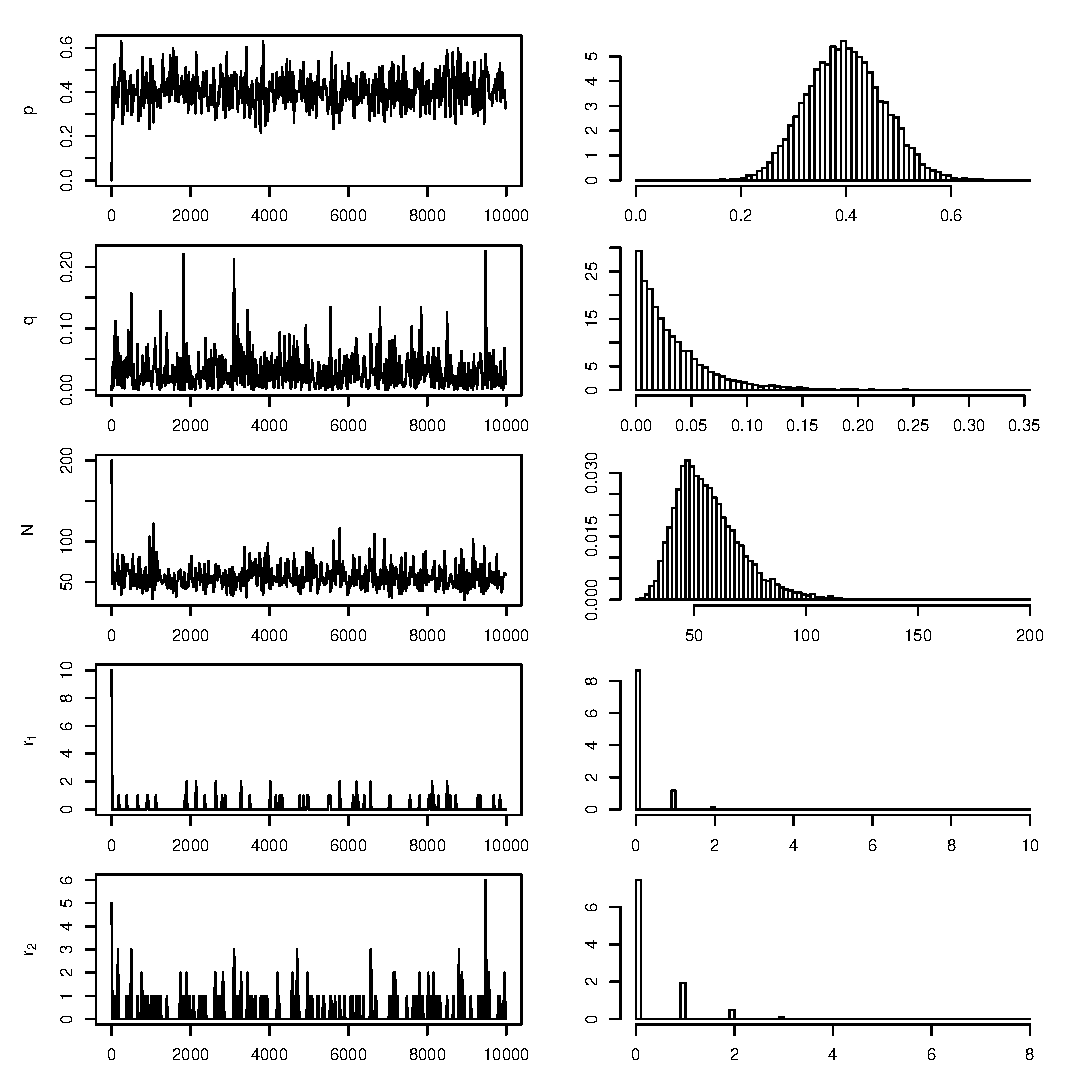
\includegraphics[width=4truecm,height=6truecm]{figures/g2.eps}}
%\only<2>{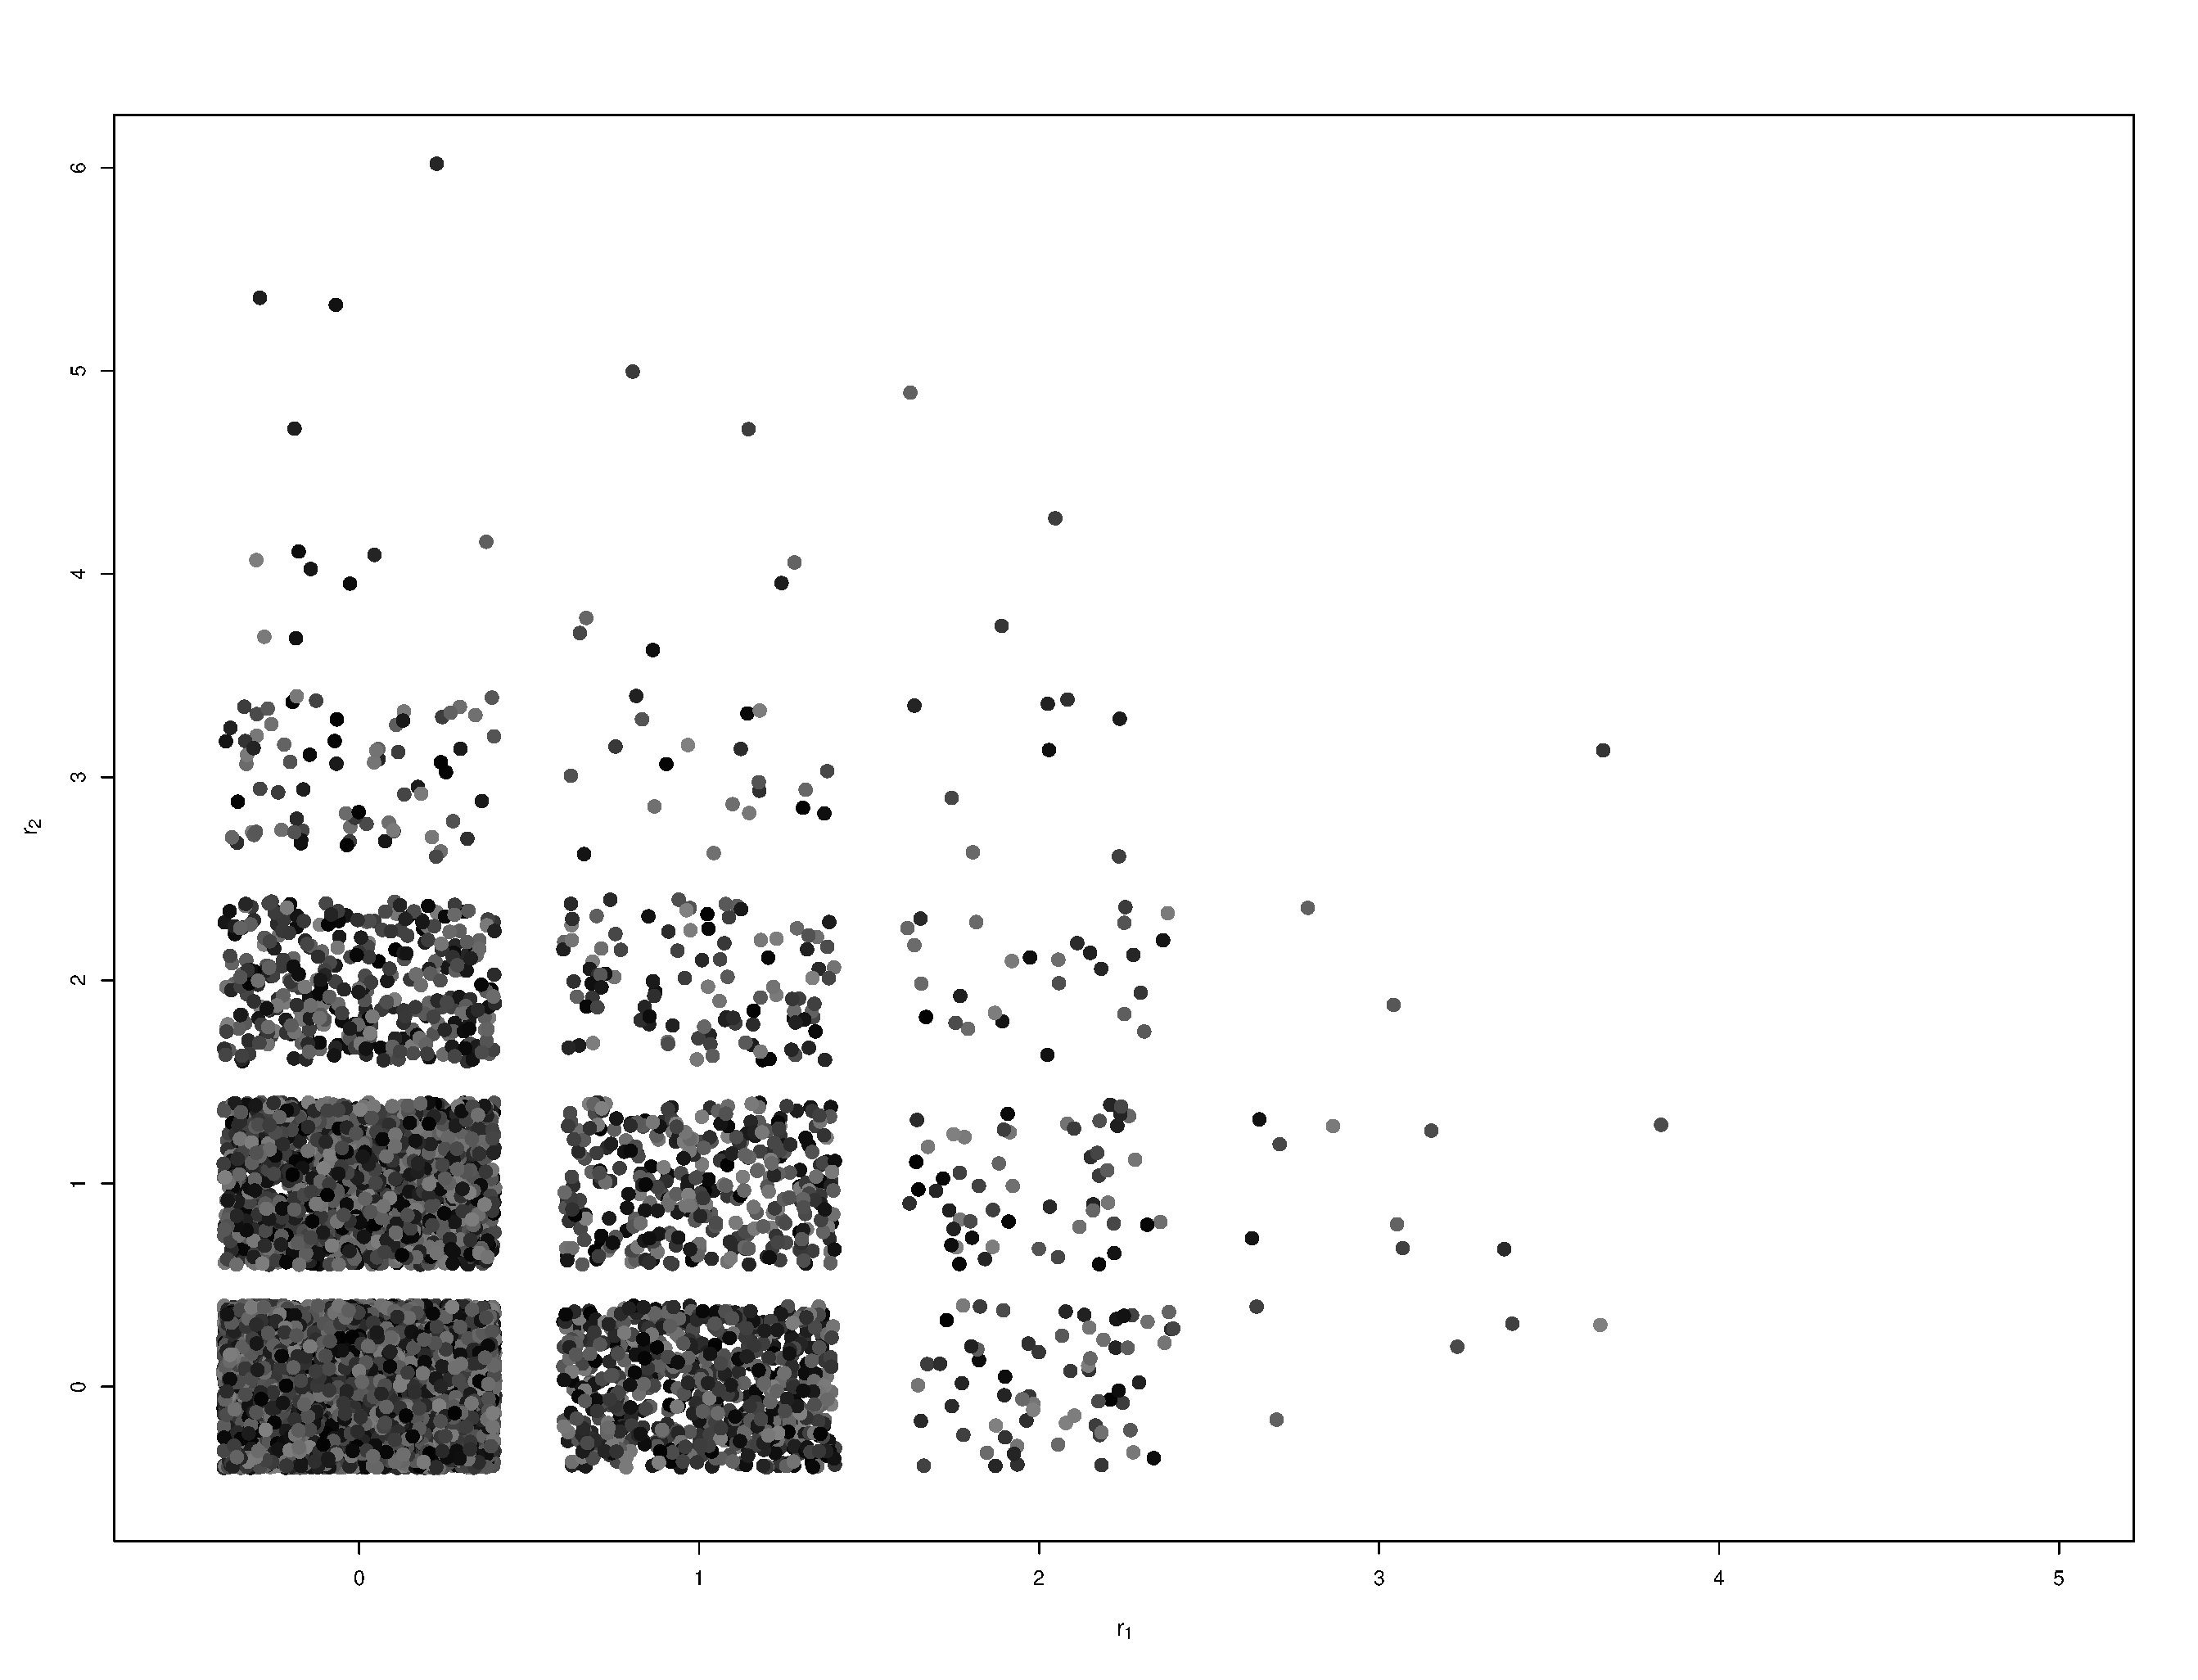
\includegraphics[width=4truecm,height=6truecm]{figures/jit.eps}}
\end{columns}

\end{slide}\begin{slide}
\slidetitle{{\sf eurodip}}

\begin{columns}
\column{.5\textwidth}
$n_1=22$, $c_2=11$ and $c_3=6$

MCMC approximations to the posterior expectations
of $N$ and $p$ equal to 57 and 0.40

\column{.5\textwidth}
%\only<1>{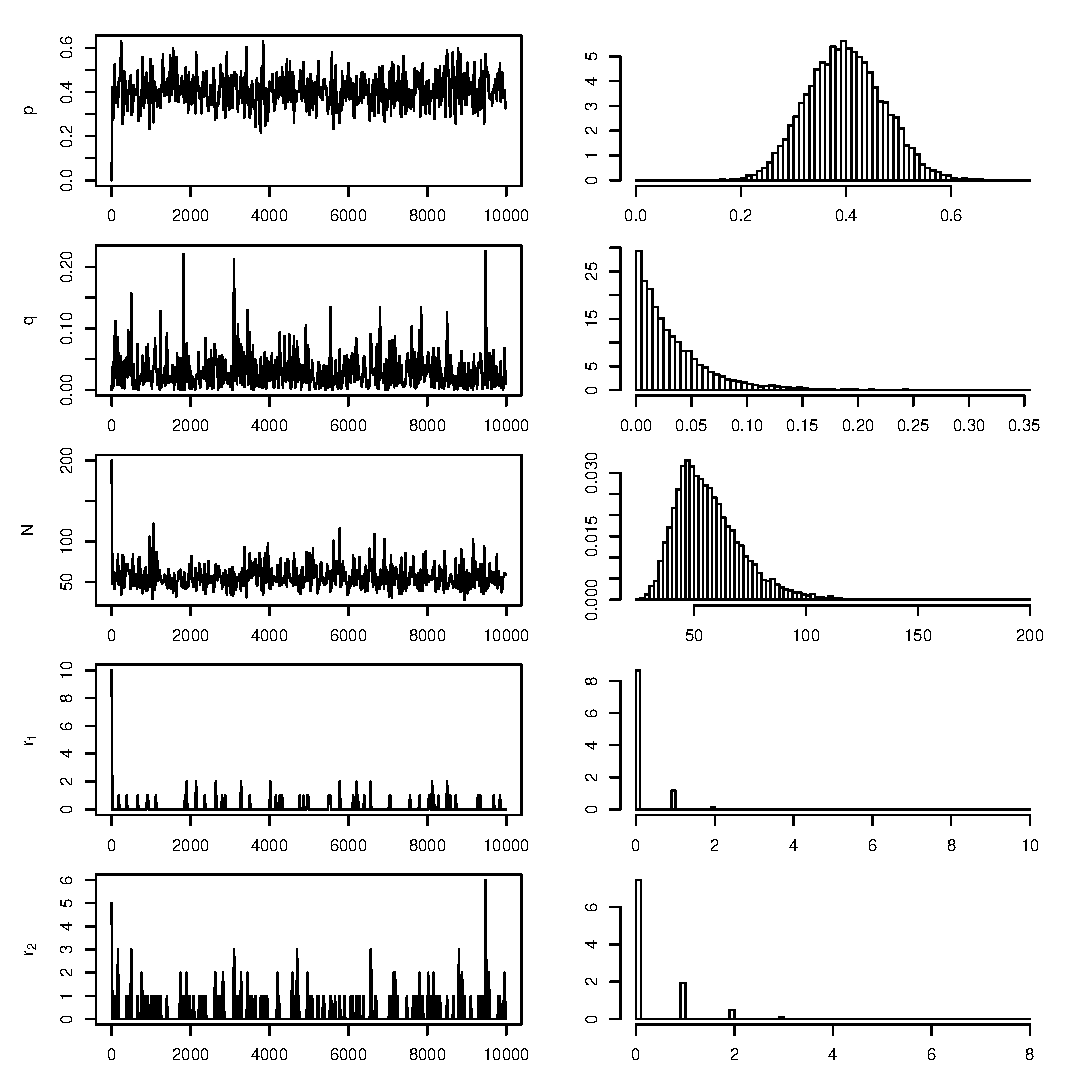
\includegraphics[width=4truecm,height=6truecm]{figures/g2.eps}}
\only<1>{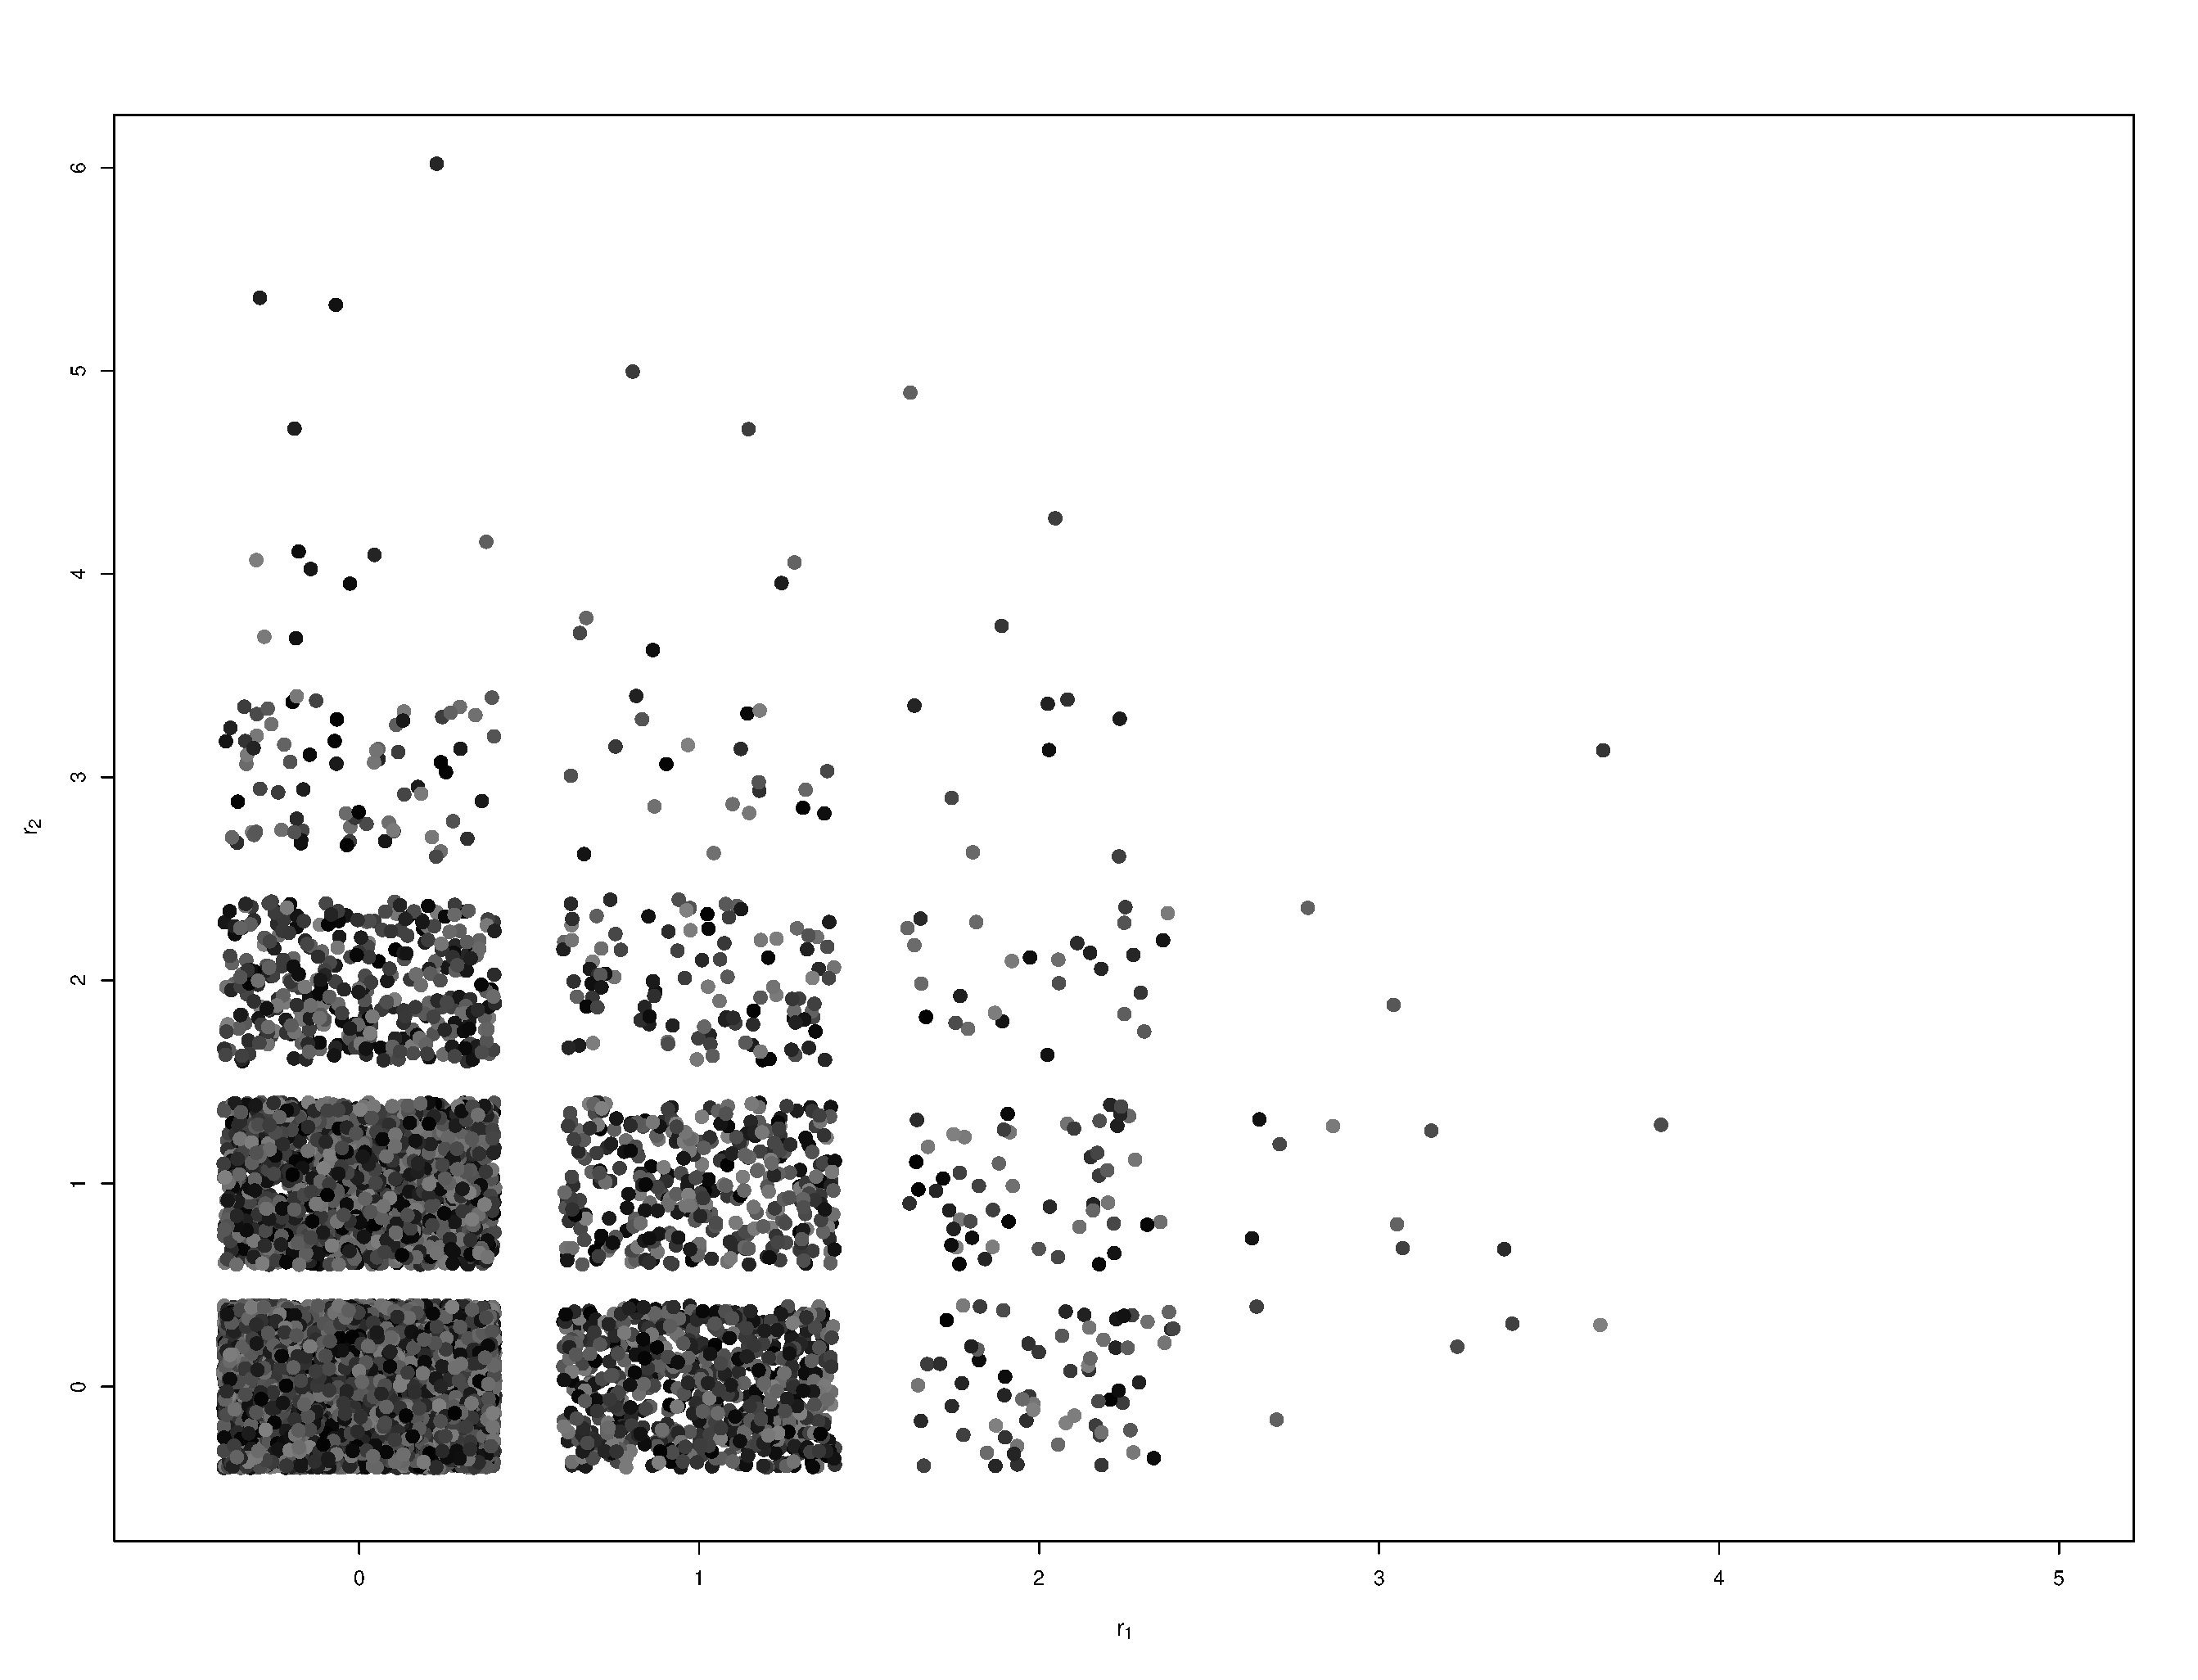
\includegraphics[width=4truecm,height=6truecm]{figures/jit.eps}}
\end{columns}

%%%%%%%%%%%%%%%%%%%%%%%%%%%%%%%%%%%%%%%
\end{slide}\subsection{Accept-Reject methods}\begin{slide}
\slidetitle{Accept-Reject methods}

\begin{itemize}
\item Many distributions from which it is difficult, or even impossible,
to directly simulate.

\item Technique that only
require us to know the functional form of the target
$\pi$ of interest up to a multiplicative constant.

\item Key to this method is to use a proposal density $g$
{\em [as in Metropolis-Hastings]}
\end{itemize}

\end{slide}\begin{slide}
\slidetitle{Principle}

Given a target density $\pi$, find a density $g$ and a constant $M$ such that
$$
\pi(x) \leq M g(x)
$$
on the support of $\pi$.

\vs\pause
Accept-Reject algorithm is then
{\Brown{\tt
\colorbox{LightGrey}{\makebox[0.9\textwidth][c]{\parbox{0.85\textwidth}{
\begin{enumerate}
\item Generate $X \sim g$, $U\sim {\cal{U}}_{[0,1]}$ ;
\item Accept $Y = X$ if $U \leq \frac{f(X) }{ Mg(X)}$ ; 
\item Return to 1.\  otherwise. 
\end{enumerate}
}}}}}

\end{slide}\begin{slide}
\slidetitle{Validation of Accept-Reject}

This algorithm produces a variable $Y$\\ distributed according to $f$

\begin{block}{Fundamental theorem of simulation}
\begin{columns}
\column{.65\textwidth}
Simulating
$$
X \sim f(x)
$$
is equivalent to simulating
$$
(X,U) \sim {\mathcal U} \{(x,u):0<u<\pi(x)\}
$$
\column{.3\textwidth}
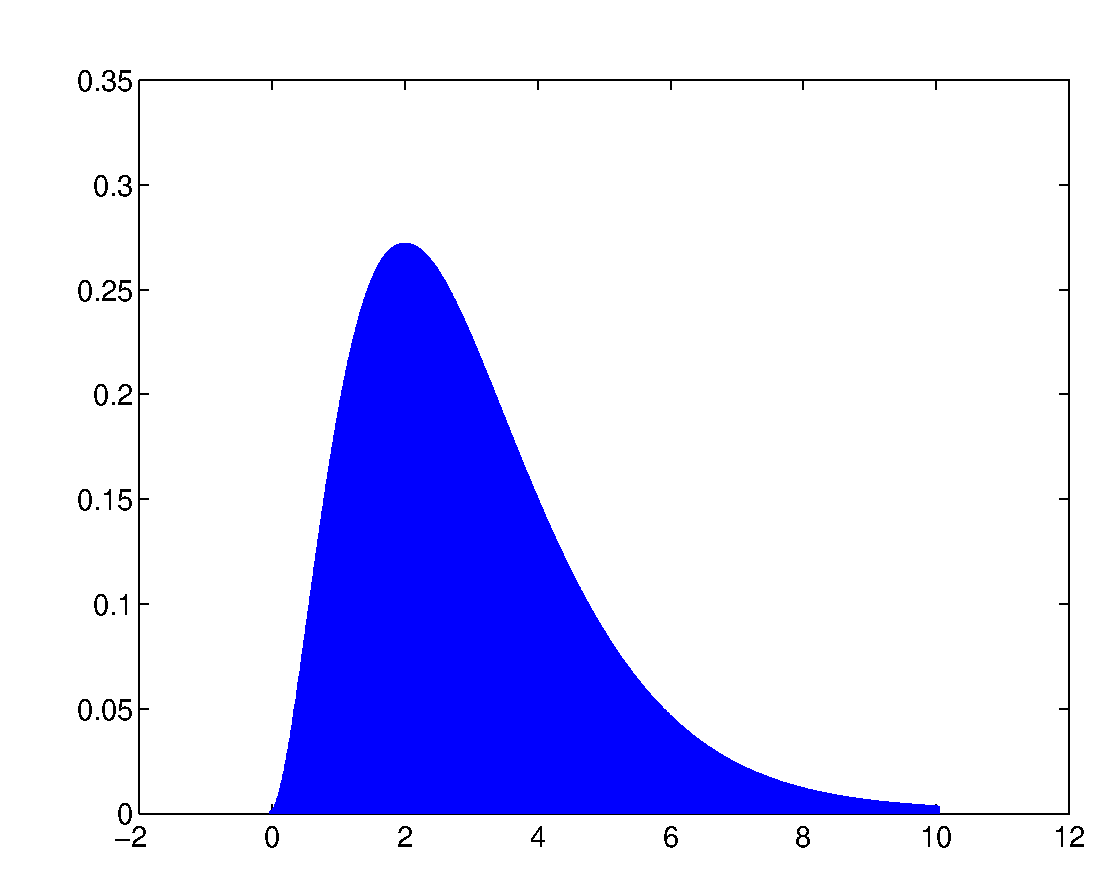
\includegraphics[width=3cm]{figures/uniform.eps}
\end{columns}
\end{block}

\end{slide}\begin{slide}
\slidetitle{Two interesting properties:}

\begin{enumerate}
\item[$\circ$] First, Accept-Reject provides a generic method 
to simulate from any density $\pi$ that is known {\it up to a multiplicative factor}

Particularly important for Bayesian calculations since
$$
  \pi(\theta|x) \propto \pi(\theta) \; f(x|\theta) \;. 
$$
is specified up to a normalizing constant
\pause
\item[$\circ$] Second, the probability of acceptance in the algorithm is $1/M$, e.g.,
expected number of trials until a variable is accepted is $M$
\end{enumerate}

\end{slide}\begin{slide}
\slidetitle{Application to the open population model}

Since full conditional distribution of $r_1$ non-standard,
rather than using exhaustive enumeration of all
probabilities $\mathbb{P}(m_1=k)=\pi(k)$ and then sampling from this distribution,
try to use a proposal based on a binomial upper bound. 

\vs\pause
Take $g$ equal to the binomial $\mathscr{B}(n_1,q_1)$ with 
$$
q_1=q/(1-q)^2(1-p)^2
$$

\end{slide}\begin{slide}
\slidetitle{Proposal bound}

$\pi(k)/g(k)$ proportional to
\footnotesize
$$
\frac{{n_1-c_2\choose k} (1-q_1)^k {n_1-k\choose r_2+c_3}}
{{n_1\choose k}} = \frac{(n_1-c_2)!}{(r_2+c_3)!n_1!}\,
\frac{((n_1-k)!)^2(1-q_1)^k}{(n_1-c_2-k)!(n_1-r_2-c_3-k)!}
$$\normalsize
decreasing in $k$, therefore bounded by
\small$$
\frac{(n_1-c_2)!}{(r_2+c_3)!}\,
\frac{n_1!}{(n_1-c_2)!(n_1-r_2-c_3)!}={n_1\choose r_2+c_3}\,.
$$\normalsize

\pause
\begin{itemize}
\item[$\lightning$] This is {\em not} the constant $M$ because of unnormalised 
densities [$M$ may also depend on $q_1$]. Therefore the average acceptance rate 
is undetermined and requires an extra Monte Carlo experiment
\end{itemize}

\end{slide}
%%%%%%%%%%%%%%%%%%%%%%%%%%%%%%%%%%%%%%%%%%%%%%%%%%%%%%%%%%%%%%%%%%%%%
\subsection{Arnason--Schwarz's Model}
\begin{slide}\slidetitle{Arnason--Schwarz Model}

\begin{columns}
\column{.55\textwidth}
Representation of a capture recapture experiment as a collection of individual histories:
for each individual captured at least once, individual characteristics
of interest (location, weight, social status, \&tc.) registered at each capture. 
\column{.4\textwidth}
\includegraphics[width=3truecm,angle=270]{figures/titlcap.eps}
\end{columns}

\vs\pause Possibility that individuals vanish from the {\em [open]} population 
between two capture experiments.

\end{slide}\begin{slide}
\slidetitle{Parameters of interest}

Study the movements of individuals between zones/strata rather than estimating
population size.

\vs\pause
Two types of variables associated with each individual $i=1,\ldots,n$

\begin{enumerate}
\item a variable for its location {\em [partly observed]},
$$
\mathbf{z}_i =(z_{(i,t)},t=1,..,\tau)
$$
where $\tau$ is the number of capture periods, 
\item a binary variable for its capture history {\em [completely observed]},
$$
\mathbf{x}_i=(x_{(i,t)},t=1,..,\tau)\,.
$$
\end{enumerate}

\end{slide}\begin{slide}
\slidetitle{Migration \&\ deaths}

$z_{(i,t)}=r$ when individual $i$ is alive in stratum $r$ at time $t$ 
and denote $z_{(i,t)}=\dag$ for the case when it is dead at time $t$.

\vs\pause Variable $\mathbf{z}_i$ sometimes called {\em migration} process of
individual $i$ as when animals moving between geographical zones.

\vs\pause
E.g., 
$$
{\mathbf x}_i = 1 \; 1 \; 0 \; 1 \; 1 \; 1\; 0 \; 0 \; 0
\quad
\text{and}
\quad
{\mathbf z}_i = 1 \; 2 \; \cdot \; 3 \; 1 \; 1 \; \cdot \; \cdot \; \cdot
$$
for which a possible completed ${\mathbf z}_i$ is
$$
{\mathbf z}_i = 1 \; 2 \; 1 \; 3 \; 1 \; 1 \; 2\; \dag \; \dag
$$
meaning that animal died between $7$th and $8$th captures 

\end{slide}\begin{slide}
\slidetitle{No tag recovery}

We assume that 
\begin{itemize}
\item $\dag$ is absorbing
\item $z_{(i,t)} =\dag$ always corresponds to $x_{(i,t)}=0$.
\item the $({\mathbf x}_i,{\mathbf z}_i)$'s ($i=1,\ldots,n$) are independent 
\item each vector ${\mathbf z}_i$ is a Markov chain on
$\mathfrak{K}\cup\{\dag\}$ with uniform initial probability on $\mathfrak{K}$.
\end{itemize}

\end{slide}\begin{slide}
\slidetitle{Reparameterisation}

Parameters of the Arnason--Schwarz model are 
\begin{enumerate}
\item capture probabilities $$\ps=\mathbb{P}\left(\xs=1|\zs=r\right)$$ 
\item transition probabilities
\small$$ \qs=\mathbb{P}\left(\zsa=s|\zs=r\right) 
\quad r\in \mathfrak{K}, s\in \mathfrak{K}\cup\{\dag\}, \quad q_t(\dag,\dag)=1
$$\normalsize
\item {\em survival} probabilities $\sos = 1 - q_t(r,\dag)$ 
\item inter-strata {\em movement} probabilities $\psi_t(r,s)$  such that
$$
\qs= \sos \times \psi_t(r,s) \quad r \in \mathfrak{K}, s \in \mathfrak{K} \,.
$$
\end{enumerate}

\end{slide}\begin{slide}
\slidetitle{Modelling}

Likelihood 
\small
\begin{align*}
 \ell(({\mathbf x}_1,{\mathbf z}_1),\ldots,({\mathbf x}_n,{\mathbf z}_n)) \propto &
 \prod_{i=1}^n\left[\prod_{t=1}^{\tau}p_t(z_{(i,t)})^{x_{(i,t)}}(1-p_t(z_{(i,t)}))^{1-x_{(i,t)}}\times\right. \nonumber\\
  &\left.\prod_{t=1}^{\tau-1}%\left(\frac{1}{\#\mathfrak{K}}\right)
q_t(z_{(i,t)},z_{(i,t+1)})\right].\label{eq:ASchwz}
\end{align*}
\normalsize

\end{slide}\begin{slide}
\slidetitle{Conjugate priors}

Capture and survival parameters
$$
\ps \sim \mathscr{B}e (a_t(r),b_t(r))\,, \qquad
\sos \sim \mathscr{B}e (\alpha_t(r),\beta_t(r))\,, 
$$
where $a_t(r),\ldots$ depend on both time $t$ and location $r$,

\pause
For  movement probabilities/Markov transitions 
$\psi_t(r) = (\psi_t(r,s); s\in\mathfrak{K})$,
$$
\psi_t(r) \sim \mathscr{D}ir (\gamma_t(r))\,,
$$
since
$$\sum_{s\in\mathfrak{K}} \psi_t(r,s)=1\,,$$
where $\gamma_t(r)= (\gamma_t(r,s); s\in\mathfrak{K})$.

\end{slide}\begin{slide}
\slidetitle{{\sf lizards}}

Capture--recapture experiment on the migrations of lizards between three adjacent zones, with
are six capture episodes. 

\vs\pause
Prior information provided by biologists on 
$p_t$ (which are assumed to be zone independent) and $\sos$, 
in the format of prior expectations and prior confidence intervals.

\vs\pause
Differences in prior on $p_t$ due to differences in capture efforts\\
differences between episodes $1,3,5$ and 
$2,4$ due to different mortality rates over winter.

\end{slide}\begin{slide}
\slidetitle{Prior information}

\footnotesize
\begin{tabular}{cl|ccccc}
\hline
&Episode  & 2   & 3    & 4   & 5  & 6 \\
\hline
$p_t$  &Mean  & 0.3  & 0.4  & 0.5  & 0.2  & 0.2 \\
&$95\% \;$ int.& [0.1,0.5]  & [0.2,0.6]  & [0.3,0.7] & [0.05,0.4] & [0.05,0.4]\\
\end{tabular}

\begin{tabular}{cl|ccc|ccc}
\hline
&Site  &       &A&  & &B,C& \\
&Episode  & t=1,3,5 & & t=2,4 & t=1,3,5 & & t=2,4 \\
\hline $\sos$
&Mean  & 0.7 & & 0.65  & 0.7 & & 0.7  \\
&$95\%\;$ int.& [0.4,0.95]& &[0.35,0.9]  & [0.4,0.95]& &[0.4,0.95]\\
\hline
\end{tabular}
\normalsize

\end{slide}\begin{slide}
\slidetitle{Prior equivalence}

Prior information that can be translated in a collection of beta priors

\pause\smallskip
\footnotesize
\begin{tabular}{l|ccccc}
\hline
Episode  & 2   & 3    & 4   & 5  & 6 \\
\hline
Dist.  & $\mathscr{B}e(6,14)$ & $\mathscr{B}e(8,12)$ & $\mathscr{B}e(12,12)$ & $\mathscr{B} e(3.5,14)$ & $\mathscr{B} e(3.5,14)$ \\
\end{tabular}

\begin{tabular}{l|ccc|ccc}
\hline
Site  &        & A &  & & B & \\
Episode  & t=1,3,5 & & t=2,4 & t=1,3,5 & & t=2,4 \\
\hline
Dist. & $\mathscr{B}e(6.0,2.5)$ &  & $\mathscr{B}e(6.5,3.5)$ & $\mathscr{B}e(6.0,2.5)$ & & $\mathscr{B} e(6.0,2.5)$ \\
\hline
\end{tabular}
\normalsize

\end{slide}\begin{slide}
\slidetitle{{\sf eurodip}} 

Prior belief that the capture and survival rates should be constant over time
$$
p_t(r)=p(r) \quad\text{and}\quad \phi_t(r)=\phi(r)
$$

\vs\pause Assuming in addition that movement probabilities are time-independent,
$$
\psi_t(r) = \psi(r)
$$
we are left with $3[p(r)]+3[\phi(r)]+3\times 2[\sos] = 12$ parameters. 

\vs\pause 
Use non-informative priors with 
$$
a(r)=b(r)=\alpha(r)=\beta(r)=\gamma(r,s)=1
$$ 

\end{slide}\begin{slide}
\slidetitle{Gibbs sampling}

Needs to account for the missing parts in the $\mathbf{z}_i$'s, in order to simulate
the parameters from the full conditional distributions
$$
\pi(\theta|\bx,\bz) \propto
\ell(\theta|\bx,\bz)\times \pi(\theta)\,,
$$
where $\bx$ and $\bz$ are the collections of the vectors of capture indicators and locations.

\vs\pause Particular case of {\em data augmentation}, where the missing
data $\bz$ is simulated at each step $t$ in order to reconstitute a complete sample $(\bx,\bz^{(t)})$
with two steps:
\begin{itemize}
\item Parameter simulation
\item Missing location simulation
\end{itemize}

\end{slide}\begin{slide}
\slidetitle{Arnason--Schwarz Gibbs sampler}

\begin{block}{Algorithm}\small
Iteration $l$ $(l\ge 1)$\index{Algorithm!Arnason-Schwarz Gibbs}
\begin{enumerate}
\item {{\bfseries Parameter simulation}}\\
simulate $\theta^{(l)} \sim \pi(\theta|\bz^{(l-1)},\bx)$ as $(t=1,\ldots,\tau)$
\begin{align*}
p_t^{(l)}(r) | \bx,\bz^{(l-1)}     & \sim \mathscr{B}e\left(a_t(r)+u_t(r),b_t(r)+ v_t^{(l)}(r)\right)\\
\phi_t^{(l)}(r) | \bx,\bz^{(l-1)}  & \sim \mathscr{B}e\left(\alpha_t(r)+ \sum_{j \in \mathfrak{K}} w_t^{(l)}(r,j),
                                                            \beta_t(r)+ w_t^{(l)}(r,\dag)\right)\\
\psi_t^{(l)}(r)| \bx,\bz^{(l-1)}   & \sim \mathscr{D}ir\left(\gamma_t(r,s)+w_t^{(l)}(r,s);s\in \mathfrak{K}\right)
\end{align*}
\end{enumerate}
\normalsize\end{block}

\end{slide}\begin{slide}
\slidetitle{Arnason--Schwarz Gibbs sampler (cont'd)}

\begin{block}\small
\begin{enumerate}
\item[ ]where
\begin{align*}
w_t^{(l)}(r,s) &=\sum_{i=1}^n \mathbb{I}_{(\zs^{(l-1)}=r,\zsa^{(l-1)}=s)} \\
u^{(l)}_t(r)   &=\sum_{i=1}^n \mathbb{I}_{(\xs=1,\zs^{(l-1)}=r)} \\
v_t^{(l)}(r)   &=\sum_{i=1}^n \mathbb{I}_{(\xs=0,\zs^{(l-1)}=r)}
\end{align*}
\end{enumerate}
\normalsize\end{block}

\end{slide}\begin{slide}
\slidetitle{Arnason--Schwarz Gibbs sampler (cont'd)}

\begin{block}\small
\begin{enumerate}
\setcounter{enumi}{1}
\item {{\bfseries Missing location simulation}}\\
generate the unobserved $\zs^{(l)}$'s from the full conditional distributions
\footnotesize
\begin{align*}
\mathbb{P}(z_{(i,1)}^{(l)}=s&|x_{(i,1)},z_{(i,2)}^{(l-1)},\theta^{(l)})
\propto q_1^{(l)}(s,z_{(i,2)}^{(l-1)})(1-p_1^{(l)}(s))\,,\\
%
\mathbb{P}(\zs^{(l)}=s&|x_{(i,t)},z_{(i,t-1)}^{(l)},z_{(i,t+1)}^{(l-1)},\theta^{(l)})
\propto q_{t-1}^{(l)}(z_{(i,t-1)}^{(l)},s)\\
&\times q_{t}(s,z_{(i,t+1)}^{(l-1)})(1-p_t^{(l)}(s))\,,\\
%
\mathbb{P}(z_{(i,\tau)}^{(l)}=s&|x_{(i,\tau)},z_{(i,\tau-1)}^{(l)},\theta^{(l)})
\propto q_{\tau-1}^{(l)}(z_{(i,\tau-1)}^{(l)},s)(1-p_\tau(s)^{(l)})\,.
\end{align*}
\end{enumerate}
\normalsize\end{block}
\end{slide}\begin{slide}
\slidetitle{Gibbs sampler illustrated} 

Take $\mathfrak{K}=\{1,2\}$, $n=4$, $m=8$ and ,for $\bx$,\\
\small\begin{center}
\begin{tabular}{r|cccccccc}
{\tt 1}$\ $&$\ $1$\ $&$\ $1$\   $&$\ \cdot\ $&$\ \cdot\ $&$\ $1$\ $&$\ \cdot\ $&$\ \cdot\ $&$\ \cdot\ $\\
{\tt 2}$\ $&$\ $1$\ $&$\ \cdot\ $&$\ $1$\   $&$\ \cdot\ $&$\ $1$\ $&$\ \cdot\ $&$\ $2$\   $&$\ $1\\
{\tt 3}$\ $&$\ $2$\ $&$\ $1$\   $&$\ \cdot\ $&$\ $1$\   $&$\ $2$\ $&$\ \cdot\ $&$\ \cdot\ $&$\ $1\\
{\tt 4}$\ $&$\ $1$\ $&$\ \cdot\ $&$\ \cdot\ $&$\ $1$\   $&$\ $2$\ $&$\ $1$\   $&$\ $1$\   $&$\ $2\\
\end{tabular}
\end{center}\normalsize

\vs
Take all hyperparameters equal to $1$

\end{slide}\begin{slide}
\slidetitle{Gibbs sampler illust'd (cont'd)} 

One instance of simulated $\bz$ is
\small\begin{center}
\begin{tabular}{cccccccc}
1$\ $&$\ $1$\ $&$\ $1$\ $&$\ $2$\ $&$\ $1$\ $&$\ $1$\ $&$\ $2$\ $&$\ ${\dag}  \\
1$\ $&$\ $1$\ $&$\ $1$\ $&$\ $2$\ $&$\ $1$\ $&$\ $1$\ $&$\ $1$\ $&$\ $2 \\
2$\ $&$\ $1$\ $&$\ $2$\ $&$\ $1$\ $&$\ $2$\ $&$\ $1$\ $&$\ $1$\ $&$\ $1 \\
1$\ $&$\ $2$\ $&$\ $1$\ $&$\ $1$\ $&$\ $2$\ $&$\ $1$\ $&$\ $1$\ $&$\ $2 \\
\end{tabular}
\end{center}\normalsize
which leads to the simulation of the parameters:
\begin{align*}
p_4^{(l)}(1) |\bx,\bz^{(l-1)} &\sim \mathscr{B}e (1+2,1+0)\\
\phi_7^{(l)}(2) |\bx,\bz^{(l-1)} &\sim \mathscr{B}e (1+0,1+1)\\
\psi_2^{(l)}(1,2)|\bx,\bz^{(l-1)} &\sim \mathscr{B}e (1+1,1+2)
\end{align*}
in the Gibbs sampler.

\end{slide}\begin{slide}
\slidetitle{{\sf eurodip}}

Fast convergence

\centerline{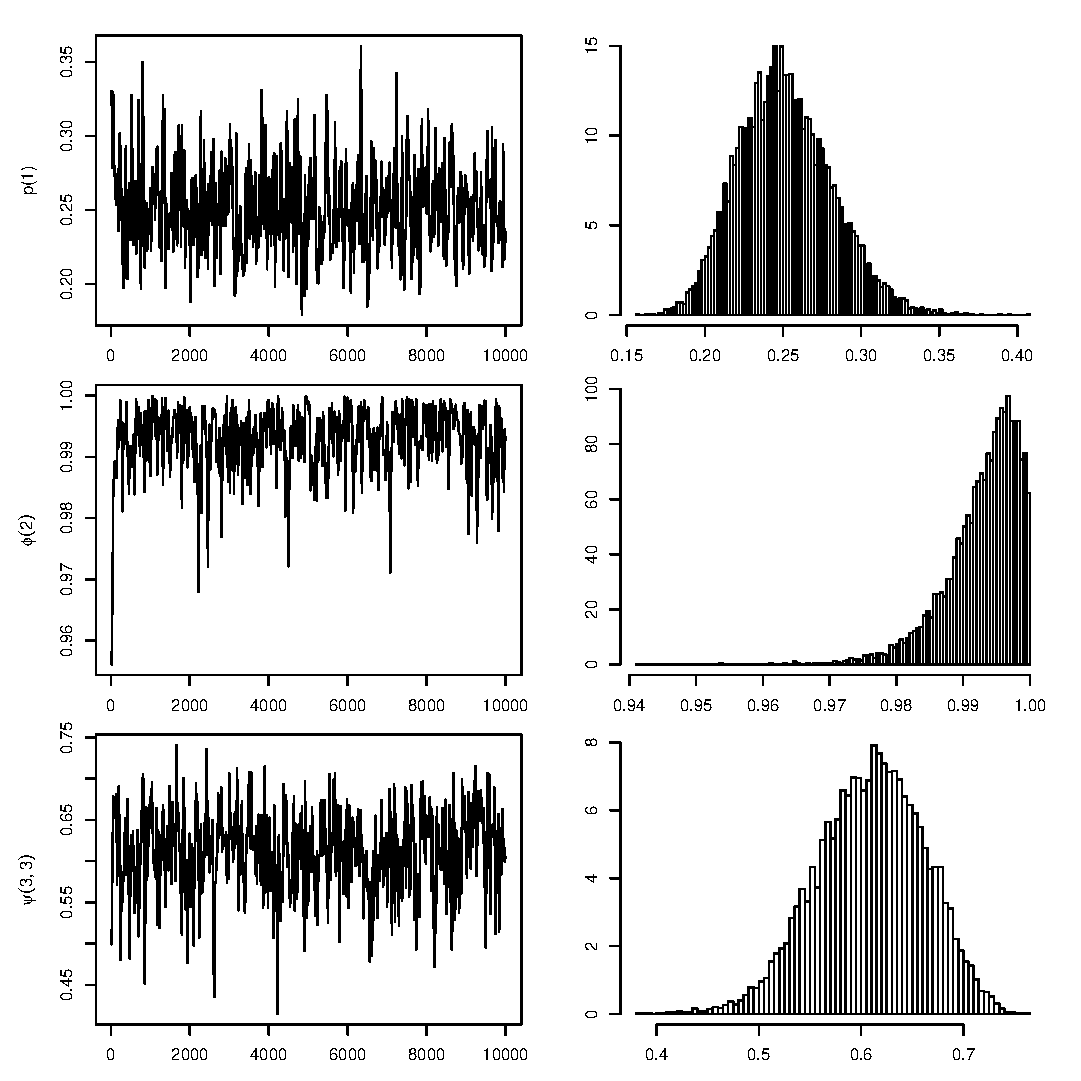
\includegraphics[width=\textwidth,height=6cm]{figures/g3.eps}}

\end{slide}
